\documentclass{tufte-handout}
\usepackage{amsmath,amsthm}

\input{vc.tex}

\usepackage{pgfplots}
%\pgfplotsset{width=\textwidth,compat=1.5.1}

\newtheorem{claim}{Claim}[section]
\title{\sf Approximation Algorithm for Maximum Cut}
%\date{\GITAuthorDate}
%\author{Thore Husfeldt}

\begin{document}

\newpage
\section{Maxcut Lab Report}


by Mats Rydberg and Martin Larsson

\subsection{Running time}

The running time of algorithm~R is $O(n+m)$.

\subsection{Randomness}

Algorithm R uses $n$ random bits.

\subsection{Solution quality}

\paragraph{Experiments.}

\begin{enumerate}
\item
For the input file  pw09\_100.9.txt with $t=100$ runs, we found
an average cutsize of $C=12320$, roughly $90,2$\% of the optimum
$\operatorname{OPT} = 13659$.
The distribution of cutsizes looks as follows:

\begin{center}

\begin{figure}
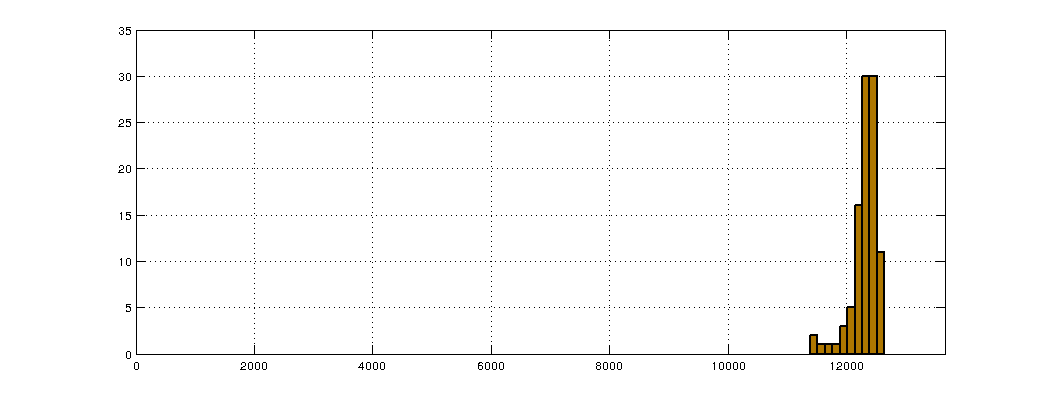
\includegraphics[scale=0.5]{hist.png}
\end{figure}

\end{center}
\medskip


\item
For the input file matching\_1000.txt with $t = 100$ runs, we found an average cutsize of $C = 252$, roughly $50,4$\% of the optimum $\operatorname{OPT} = 500$. The distribution of cutsizes looks as follows:

\begin{center}

\begin{figure}
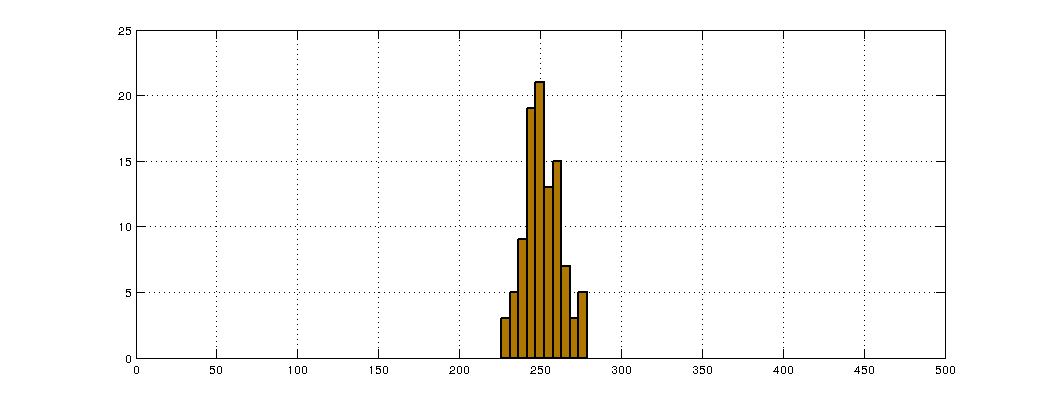
\includegraphics[scale=0.5]{hist2.png}
\end{figure}

\end{center}


\end{enumerate}
\paragraph{Analysis of performance guarantee}

Clearly, Algorithm R performs quite badly on input 
  matching\_1000.txt.
We will show that it can perform \emph{no worse} than that, i.e., we
will establish that in expectation, the cutsize $C$ satisfies $C \geq
\frac{1}{2}\cdot \operatorname{OPT}$.


We will view $C$ as a random variable that gives the size of the cut
defined by the random choices.
Let $W$ denote the total weight of the edges of $G$, i.e.,
\[ W= \sum_{e\in E} w(e)\,.\]

Then,
$$
E[C] = \textstyle\frac{1}{2}\cdot W\,.
$$

To see this, define the indicator random variable $X_{uv}$ for every
edge $uv\in E$ as follows.
Set $X_{uv}=1$ if $uv$ crosses the cut, i.e., $u\in A$ and $v\notin A$
or $u\notin A$ and $v\in A$.
Otherwise, $X_{uv} = 0$.

Then, $\Pr(X_{uv} = 1) =  \frac{1}{2}$, because either both $u$ and $v$ are in $A$, both are in $B$, or one is in $A$ and one is in $B$ (two combinations). This gives us 2 possible cuts out of 4 possible, equally likely and disjunct outcomes (clearly, $u$ and $v$ can not both be in $A$ while $v$ is in $B$) $\Rightarrow $ probability of cut is $\frac{2}{4} = \frac{1}{2}$.
Now, $$E[X_{uv}] = \sum_{k=0}^1k\cdot\Pr(X_{e} = k) = 0\cdot\frac{1}{2} + 1\cdot\frac{1}{2} = \frac{1}{2}$$
and
$$E[C]= E[\sum_{e\in E}X_{e}\cdot w(e)] = \sum_{e\in E}w(e)\cdot E[X_{e}] = \sum_{e\in E}w(e) \cdot \frac{1}{2} = \frac{1}{2}\sum_{e\in E}w(e) = \frac{1}{2}\cdot W$$ Finally, we have 
\(E[C]\geq \frac{1}{2}\cdot \text{OPT}\) because clearly
$\operatorname{OPT} \leq W$, if and only if all weights are positive.


\newpage
\section{Optional: Derandomising Algorithm R}

\subsection{Algorithm L} 


We now reduce the number of random bits used by the algorithm to $\log
n$ using a simple \emph{pseudorandom generator}.


Let $k=\lceil\log (n+1)\rceil$ and flip $k$ coins $b_1,\ldots, b_k$.
There are $2^k -1 \geq n$ different ways of choosing a nonempty subset
$S\subseteq [k]$ of the coins.
Each of these ways defines a random bit $r_S =\bigoplus_{i\in S} b_i$.
This gives a total of $n$ random bits.
These random bits are not as high-quality as the original $k$ bits,
but they retain the crucial property of \emph{pairwise independence}:
If $S\neq T$ then 
$$ \Pr(r_S\neq r_T) = \Pr(r_S=1)\cdot\Pr(r_T=0)+\Pr(r_S=0)\cdot\Pr(r_T=1)$$

Now we conclude that $\Pr(r_V=0) = \Pr(r_V=1)$ since the $b_i$ die rolls are $0$ and $1$ with equal probability ($\frac{1}{2}$), and $b_i \oplus b_j$ preserves these probabilities.

We now extend Algorithm~R using this idea; calling the resulting
algorithm~L (for logarithmic randomness).

\subsection{Algorithm Z}

For our final trick, we let the random bits disappear completely:
since Algorithm~L uses only $k$ bits of randomness, we can iterate
over \emph{all} coin flips---there are only $2^k$, which is polynomial
(in fact, linear) in $n$.
Extend algorithm~L using this idea; call the resulting algorithm~Z
(for zero randomness).
The running time of Z is $O([\ldots])$.

\newpage
\section{Perspective}

This lab establishes minimal skills in algorithms implementation,
probabilistic analysis of algorithms (independence, linearity of
expectation, and in particular the trick of computing an expectation
using indicator random variables), and approximation guarantees (in
particular, finding upper and lower bounds by exhibiting a concrete
``bad instance'' and a comparison to a hypothetical optimum,
respectively).
The histogram aims to establish the intuition that measure is
concentrated around its expectation.

\bigskip

To establish that Maxcut is NP-hard one reduces from NAE-Sat, a
reduction that can be found in many places\sidenote{C. Moore and
S. Mertens, \emph{The Nature of Computation}, Oxford University Press,
  2011, p. 146.}
Recall that the related problem \emph{Minimum Cut} is easy because of
the max flow--min cut theorem.
A moment's thought should convince you that as soon as negative
weights are allowed, the two problems are the same (and both are
hard).
Algorithm R doesn't work at all for negative weights.

Algorithm R is a classical randomised approximation algorithm, its
origins seem to be shrouded in the mists of time.
The \emph{deterministic} algorithm of Sahni and Gonzales\sidenote{S.\
  Sahni and T.\ Gonzalez.
  P-complete approximation problems.
  \emph{J.\ Assoc.\ Comput.\ Mach.}, 23(3):555--565, 1976.}
can be viewed as a derandomisation of R using the \emph{method of
  conditional expectations}.
These algorithms were best knows until the breakthrough result of
Goemans and Williamson,\sidenote{M.\ X.\ Goemans and D.\ P.\
  Williamson.
  Improved approximation algorithms for maximum cut and satisfiability
  problems using semidefinite programming.
  \emph{J.\ Assoc.\ Comput.\ Mach.}, 42(6):1115--1145, 1995.}
which improved the approximation factor to $0.87856$.
H\aa{}stad has shown that no algorithm can approximate the maxcut
better than $16/17\sim 0.941176$ unless P equals NP. Khot has shown
that the Goemans--Williamson bound is essentially optimal under the
\emph{Unique Games Conjecture}.

Algorithm L can also be viewed as an application of \emph{pairwise
  independent hash functions}.


\end{document}
